% the template is adapted from https://github.com/kourgeorge/arxiv-style

\documentclass{article}


\usepackage{arxiv}

\usepackage[usenames,dvipsnames]{xcolor} % Why it should be listed before line 16??? https://tex.stackexchange.com/questions/87197/latex-error-option-clash-for-package-xcolor-for-table


\usepackage[utf8]{inputenc} % allow utf-8 input
\usepackage[T1]{fontenc}    % use 8-bit T1 fonts
\usepackage{hyperref}       % hyperlinks
\usepackage{url}            % simple URL typesetting
\usepackage{booktabs}       % professional-quality tables
\usepackage{amsfonts}       % blackboard math symbols
\usepackage{nicefrac}       % compact symbols for 1/2, etc.
\usepackage{microtype}      % microtypography
\usepackage{lipsum}		% Can be removed after putting your text content

\usepackage{tikz} 
\usetikzlibrary{matrix}

\usepackage{graphicx}
%\usepackage{hyperref}
\usepackage{amsmath,amssymb}
\usepackage{algorithm}
%\usepackage{algorithmicx}
%\usepackage{algpseudocode}
\usepackage{subcaption}
%\usepackage{booktabs}

\usepackage{listings}
%\usepackage[T1]{fontenc}
%\usepackage{beramono}


%%
%% Julia definition (c) 2014 Jubobs
%%
\lstdefinelanguage{Julia}%
  {morekeywords={abstract,break,case,catch,const,continue,do,else,elseif,%
      end,export,false,for,function,immutable,import,importall,if,in,%
      macro,module,otherwise,quote,return,switch,true,try,type,typealias,%
      using,while},%
   sensitive=true,%
   alsoother={\$},%
   morecomment=[l]\#,%
   morecomment=[n]{\#=}{=\#},%
   morestring=[s]{"}{"},%
   morestring=[m]{'}{'},%
}[keywords,comments,strings]%

\lstset{%
    language         = Julia,
    basicstyle       = \ttfamily,
    keywordstyle     = \bfseries\color{blue},
    stringstyle      = \color{magenta},
    commentstyle     = \color{ForestGreen},
    showstringspaces = false,
}




\title{Some not that novel approach to image processing using nonparametric statistic}


%\date{September 9, 1985}	% Here you can change the date presented in the paper title
%\date{} 					% Or removing it

\author{
  Zhuo Yueyi \\ %\thanks{Use footnote for providing further
    %information about author (webpage, alternative
    %address)---\emph{not} for acknowledging funding agencies.} \\
  Department of Computer Science and Engineering\\
  Nanjing University of Science and Technology\\
  \texttt{yiyuezhuo@gmail.com} \\
}

\begin{document}
\maketitle

\begin{abstract}
%\lipsum[1]
This is a class paper for nonparametric statistical. 
Some methods introduced by \cite{wasserman2006all} will get a example to show how it can be applied on
image processing problem, such as kernel regression, local polynomial regression, cross validation, variance estimation
by smoothing, histogram, kernel density estimation density estimation using regression and bootstrap.
\end{abstract}


% keywords can be removed
\keywords{Nonparametric statistic \and image processing }


\section{Introduction}
%\lipsum[2]
%\lipsum[3]




\subsection{Data format of image}
%\label{sec:headings}
%\lipsum[4] See Section \ref{sec:headings}.

Colored(RGB) image can be seen as a 3 variables function  $f(i,j,c)$, where $i,j$ denote the location of image, $c$ denotes
channel(red, green, blue). The function can be encoded by three matrixes as shown in Fig~\ref{fig:toad_rgb}.

\begin{figure}[htb]
  \centering
  \begin{tikzpicture}
    \node[inner sep=0pt] (toad_rgb) at (-2.5,0)
    {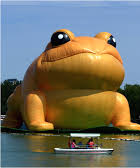
\includegraphics[width=.15\textwidth]{images/toad_rgb.png}};
    \node[inner sep=0pt] (toad_r) at (0.0,0)
    {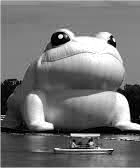
\includegraphics[width=.15\textwidth]{images/toad_r.png}};
    \node[inner sep=0pt] (toad_g) at (2.5,0)
    {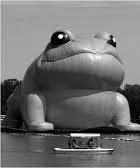
\includegraphics[width=.15\textwidth]{images/toad_g.png}};
    \node[inner sep=0pt] (toad_b) at (5.0,0)
    {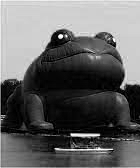
\includegraphics[width=.15\textwidth]{images/toad_b.png}};
    
    \draw [->] (toad_rgb.south) to [out=355, in=185] (toad_r.south);
    \draw [->] (toad_rgb.south) to [out=350, in=190] (toad_g.south);
    \draw [->] (toad_rgb.south) to [out=345, in=195] (toad_b.south);

    % small crop in toad_b
    %\draw [red] (7.5, 0.05) -- (7.6, 0.05) -- (7.6,-0.05) -- (7.5, -0.05) -- (7.5, 0.05);
    \draw [red] ([shift={(0.0, 0.05)}]toad_b.center) --
      ([shift={(0.1, 0.05)}]toad_b.center) --
      ([shift={(0.1, -0.05)}]toad_b.center) --
      ([shift={(0.0, -0.05)}]toad_b.center) --
      ([shift={(0.0, 0.05)}]toad_b.center);

    %\node (10.0,0.0) {$$\begin{bmatrix} 1 & 1 \\ 2 & 2 \end{bmatrix}$$};
    \matrix [matrix of nodes,row sep=-1ex, column sep=-1ex] (toad_mat) at (7.7, 0.0)
    {
        5 & 7 & 10 & 10 & 11 & 4 \\
        6 & 8 & 8 & 10 & 10 & 5 \\
        5 & 6 & 8 & 8 & 7 & 4 \\
        6 & 5 & 6 & 5 & 7 & 5 \\
        6 & 6 & 4 & 5 & 4 & 4 \\
        5 & 5 & 4 & 2 & 3 & 6  \\  };

    \draw [->] ([shift={(0.1, 0.05)}]toad_b.center) -- (toad_mat.north west);
    \draw [->] ([shift={(0.1, -0.05)}]toad_b.center) -- (toad_mat.south west);

    % draw matrix frame, how stupid I need to write it manually.
    \draw ([shift={(0.15, 0.0)}]toad_mat.north west) -- 
        ([shift={(0.05, 0.0)}]toad_mat.north west) --
        ([shift={(0.05, 0.0)}]toad_mat.south west) --
        ([shift={(0.15, 0.0)}]toad_mat.south west);

    \draw ([shift={(-0.15, 0.0)}]toad_mat.north east) -- 
        ([shift={(-0.05, 0.0)}]toad_mat.north east) --
        ([shift={(-0.05, 0.0)}]toad_mat.south east) --
        ([shift={(-0.15, 0.0)}]toad_mat.south east);

    \node at ([shift={(0.0, 0.2)}]toad_rgb.north) {RGB};
    \node at ([shift={(0.0, 0.2)}]toad_r.north) {R};
    \node at ([shift={(0.0, 0.2)}]toad_g.north) {G};
    \node at ([shift={(0.0, 0.2)}]toad_b.north) {B};
    \node at ([shift={(0.0, 0.2)}]toad_mat.north) {matrix of the crop};
    
    % two example equation to show the function sematic
    \node (eq1) at  (10.0, 0.2) {$f(84, 72, 2)$};
    \node (eq2) at  (10.0,-0.2) {$f(85, 72, 2)$};

    \draw [->] ([shift={(-0.2, 0.2)}]toad_mat.east) -- (eq1);
    \draw [->] ([shift={(-0.2, -0.2)}]toad_mat.east) -- (eq2);

    %\draw[help lines] (0,0) grid (10,-10);
\end{tikzpicture}

  \caption{Representation: Image as three matrix}
  \label{fig:toad_rgb}
\end{figure}

Since the colored image introduce extra complexity, in most of this paper, the gray image is used for simplicity.
Instead of three matrices, the gray image is represented by a single matrix which is given by:

\begin{equation}
  f_{gray}(i,j) = 0.21 f_{rgb}(i,j,1) + 0.72 f_{rgb}(i,j,2) + 0.07 f_{rgb}(i,j,3)
  \label{eq:rgb_to_gray}
\end{equation}

Sometimes "flattening" a matrix to a long vector is a useful viewpoint. There're two order to flatten a matrix,
row-major and column-major. The row-major is used in Python(Numpy) and the column-major is used by R,Julia and MatLab.
Row-major order of Python is illustrated as Fig~\ref{fig:flatten_matrix}.

\begin{figure}[htb]
  \centering
  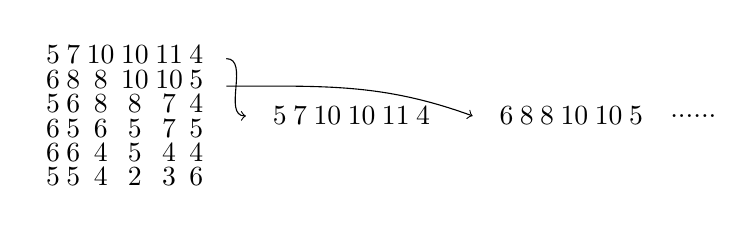
\begin{tikzpicture}
    \matrix [matrix of nodes,row sep=-1ex, column sep=-1ex, anchor=west] (toad_mat) at (0.0, 0.0)
    {
        5 & 7 & 10 & 10 & 11 & 4 \\
        6 & 8 & 8 & 10 & 10 & 5 \\
        5 & 6 & 8 & 8 & 7 & 4 \\
        6 & 5 & 6 & 5 & 7 & 5 \\
        6 & 6 & 4 & 5 & 4 & 4 \\
        5 & 5 & 4 & 2 & 3 & 6  \\  };
    
    \matrix [matrix of nodes,row sep=-1ex, column sep=-1ex, anchor=west] (toad_r1) at ([shift={(0.4, 0.00)}]toad_mat.east)
    {
        5 & 7 & 10 & 10 & 11 & 4 \\};

    \matrix [matrix of nodes,row sep=-1ex, column sep=-1ex, anchor=west] (toad_r2) at ([shift={(0.4, 0.00)}]toad_r1.east)
    {
        6 & 8 & 8 & 10 & 10 & 5 \\};
    
    \node (ellipsis) at  ([shift={(0.4, 0.00)}]toad_r2.east) {......};

    %\draw [->] ([shift={(0.05, 0.00)}]toad_mat.east ) -- ([shift={(-0.1, 0.00)}]toad_r1.west);
    %\draw [->] ([shift={(0.05, -0.60)}]toad_mat.east ) -- ([shift={(-0.1, 0.00)}]toad_r2.west);
    \draw [->] ([shift={(0.05, -0.40)}]toad_mat.north east) to [out=0, in=180] ([shift={(-0.1, 0.00)}]toad_r1.west);
    \draw [->] ([shift={(0.05, -0.75)}]toad_mat.north east) to [out=0, in=160] ([shift={(-0.1, 0.00)}]toad_r2.west);

\end{tikzpicture}

  \caption{Flatten a matrix by row}
  \label{fig:flatten_matrix}
\end{figure}


As a application we can model the vector as i.i.d sample of some distribution using simpler symbol, the most 
common practice is to represent them as a histogram, see Fig~\ref{fig:map_gray_to_hist}. 
For more detail, refer to Section~\ref{segmentation}.

\begin{figure}[htb]
  \centering
  \begin{tikzpicture}
    \node[inner sep=0pt, anchor=west] (toad_gray) at (0,0)
    {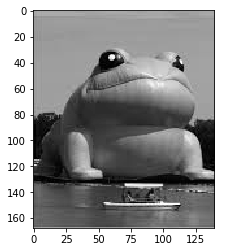
\includegraphics[width=.15\textwidth]{images/toad_gray.png}};
    \node[inner sep=0pt, anchor=west] (toad_hist) at ([shift={(0.5, 0.0)}]toad_gray.east)
    {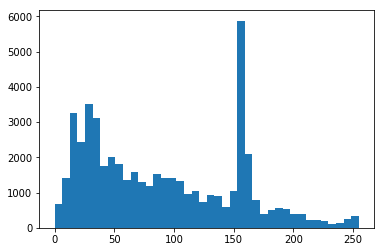
\includegraphics[width=.15\textwidth]{images/toad_hist.png}};

    \draw [->] (toad_gray.east) -- (toad_hist.west);

\end{tikzpicture}

  \caption{Mapping from gray image to histogram}
  \label{fig:map_gray_to_hist}
\end{figure}

\subsection{Inverse problem in image processing}

As presented in \cite{dong2015image}, we usually regard image as a result of combination of some "observe"
function and noise. In its simplest form, we can write:

\begin{equation}
\mathbf{f} = \mathbf{A} \mathbf{x} + \mathbf{\eta}
\label{eq:inverse_problem}
\end{equation}

where $\mathbf{f}$ denote a (gray) image, $\mathbf{A}$ is a linear operation(usually a convolution)
\footnote{This equation can be written as a verbose conventional matrix equation, 
see document of MatLab function \bf{im2col}}, 
$\mathbf{x}$ is "true" image, $\mathbf{\eta}$ is noise term.
 
\section{Smoothing: nonparametric statistic and image processing}

There exists a fully equivalence which can be shown on smoothing problem.

\cite{wasserman2006all} state regression for pairs $((x_1,Y_1),\dots,(x_n,Y_n))$ like:

$$
Y_i = r(x_i) + \epsilon_i
$$

Replacing $x_i$ with $x_{ij}=(i,j)$ ($i,j$ denote coordinates of corresponding pixel on image), compared to Eq~\ref{eq:inverse_problem},
so the $r(x_{i,j})=r(i,j)$ denote the complex true image function. $\epsilon_i \to \epsilon_{i,j} \sim N(0,\sigma)$ is i.i.d white noise.
It's obvious that we can not specify a simple parametric model on it (For some possible parametric image model,
see Fig~\ref{fig:parametric_model} ) so that the noise derived from underestimated model will cause misunderstanding. 
Thus we must employ a nonparametric fashion though computer scientist may not aware it explicitly.

\begin{figure}[htb]
  \centering
  \begin{subfigure}[b]{0.24\linewidth}
    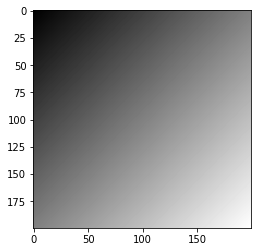
\includegraphics[width=\linewidth]{images/parametric_model_1.png}
    \caption{$y_{ij} = i+j$}
  \end{subfigure}
  \begin{subfigure}[b]{0.24\linewidth}
    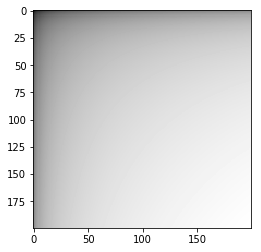
\includegraphics[width=\linewidth]{images/parametric_model_2.png}
    \caption{$y_{ij} = \log(1+i)+\log(1+j)$}
  \end{subfigure}
  \begin{subfigure}[b]{0.24\linewidth}
    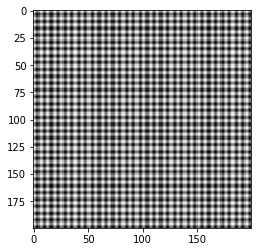
\includegraphics[width=\linewidth]{images/parametric_model_3.png}
    \caption{$y_{ij} = \sin(i)+\sin(j)$}
  \end{subfigure}
  \begin{subfigure}[b]{0.24\linewidth}
    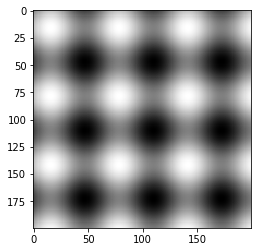
\includegraphics[width=\linewidth]{images/parametric_model_4.png}
    \caption{$y_{ij} = \sin(0.1i)+\sin(0.1j)$}
  \end{subfigure}
  \caption{Simple parametric model can't capture big picture of image.}
  \label{fig:parametric_model}
\end{figure}


\subsection{Kernel regression}
%\lipsum[5]
%\begin{equation}
%\xi _{ij}(t)=P(x_{t}=i,x_{t+1}=j|y,v,w;\theta)= {\frac {\alpha _{i}(t)a^{w_t}_{ij}\beta _{j}(t+1)b^{v_{t+1}}_{j}(y_{t+1})}{\sum _{i=1}^{N} \sum _{j=1}^{N} \alpha _{i}(t)a^{w_t}_{ij}\beta _{j}(t+1)b^{v_{t+1}}_{j}(y_{t+1})}}
%\end{equation}

As stated in \cite{solomon2011fundamentals}, a mean filtering, as simplest filter technology, give same weight to neibor pixel to smooth the
noised to remove noise(try to find true $r(i,j)$ ). Concretely, here's a instance of $3 \times 3$ filtering:

\begin{equation}
g(i,j) = \frac{1}{9} \sum_{di=-1}^1 \sum_{dj=-1}^1 f(i+di,j+dj)
\label{eq:mean_filter}
\end{equation}

If we set kernel function as:

$$ 
K(x_{i,j},y_{i,j}) =  
\begin{cases}
  1, & \text{if $ |i_x - i_y| \le 1$ and $|j_x - j_y| \le 1$} \\
  0, & \text{otherwise}
\end{cases}
$$

Which is a nature two-variables extension from box-car kernel introduced by \cite{wasserman2006all}.
Then the kernel regression given by:

$$
\hat{r}(x_{i,j}) = \frac{\sum_{s} \sum_{t} K(x_{i,j},x_{s,t}) Y_{s,t}}{\sum_{s} \sum_{t} K(x_{i,j},x_{s,t})}
$$

is equivalence to Eq~\ref{eq:mean_filter}. A example can be shown in Fig~\ref{fig:effect_noise_removal}. 
The kernel size(here it's $3$) is directly correspond to bandwidth $h$ used in kernel regression. 
We can see that $h=5$(mean kernel = $11 \times 11 $) lead to over-smooth $\hat{r}$, $h=1$ seems under-smoothed,
while the result of median seems fine.

Mean filtering is usually weaker than median filtering, a example is shown in Fig~\ref{fig:effect_noise_removal}. 
Though median filtering is also a linear smoother: 

$$
\hat{r}(x_{i,j})=\sum_s \sum_t l_{s,t}(x_{i,j})Y_{s,t}$$

its hat-"matrix"(here is 4d tensor) can be represented as: 

$$ 
l_{s,t}(x_{i,j}) = I(s=i_{median}) \times I(t=j_{median}) 
$$

Where $i_{median},j_{median}$ denote the coordinates of pixel which is median of neighborhood of given pixel $(i,j)$.

But obviously it can not be included by kernel regression, say, 
we can't find a general kernel function $K(x_{i,j},y_{i,j})$ which give above hat matrix. 

Following textbook \cite{wasserman2006all}, we can try to find different improvement other than mean-filter 
(i.e. gaussian kernel regression(filtering) using gaussian kernel) rank-filter, or, 
for example, local polynomial regression. 

\begin{figure}[htb]
  \centering
  \begin{subfigure}[b]{0.24\linewidth}
    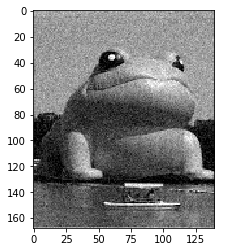
\includegraphics[width=\linewidth]{images/noise_removal_1.png}
    \caption{Noised toad}
  \end{subfigure}
  \begin{subfigure}[b]{0.24\linewidth}
    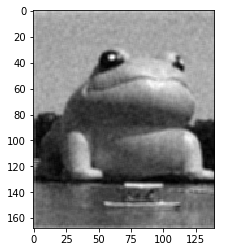
\includegraphics[width=\linewidth]{images/noise_removal_2.png}
    \caption{Kernel regression(h=1)}
  \end{subfigure}
  \begin{subfigure}[b]{0.24\linewidth}
    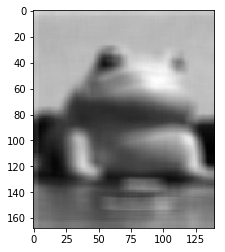
\includegraphics[width=\linewidth]{images/noise_removal_3.png}
    \caption{Kernel regression(h=5)}
  \end{subfigure}
  \begin{subfigure}[b]{0.24\linewidth}
    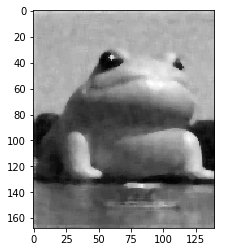
\includegraphics[width=\linewidth]{images/noise_removal_4.png}
    \caption{Median regression(h=3)}
  \end{subfigure}
  \caption{$\hat{r}(x_{i,j})$}
  \label{fig:effect_noise_removal}
\end{figure}


\subsection{Local Polynomial Regression}

Basically, polynomial regression fit a "delta" model $f_{i,j}(di,dj)$ for every points $(i,j)$, and use $f(0,0)$
as estimation of $\hat{r}(x_{i,j})$. Especially, the linear formulation with kernel weighting is most 
interesting considering higher order may causing numerical problem.

The vanilla equation:

$$
\mathbf{l}(x) = e_1^T (X_x^T W_x X_x)^{-1} X_x^T W_x
$$

may lead too large matrix $W_x$ ($23520 \times 23520$), so the broadcast trick is used to represent the matrix as 
$23520$ vector. However, fit a model $23520$ times using slightly different parameters is inevitable. 
The result seems nice more than results given by kernel regression and median filter, 
as shown in Fig~\ref{fig:local_poly} \footnote{The above related code is written in Python and following related code is written in Julia}.  
The "true" means that the model is applied on true image instead of noised image,
we can see the detail is kept finely compared to other methods which may over-smooth even in "true" image.
The right one show $h=1$ result of smoothing the noised image, we can see the result may not be better than median regression especially considering
it costly computation time. 

And it can also provide variance information. The second sub-fig show the value of linear, it show the linear
"trend" in that pixel. Taking absolute on it, we can compare it to so called edge detection filter such as Sobel operation and LoG
in image processing, see Fig~\ref{fig:edge}. It's reasonable since the edge is so called high frequency feature, hence the extremely
change matched by different methods will give consistent response as seen in those figures.

\begin{figure}[htb]
  \centering
  \begin{subfigure}[b]{0.24\linewidth}
    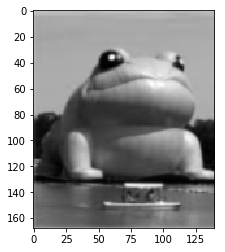
\includegraphics[width=\linewidth]{images/poly_nr.png}
    \caption{Local Poly Reg Cons(true)}
  \end{subfigure}
  \begin{subfigure}[b]{0.24\linewidth}
    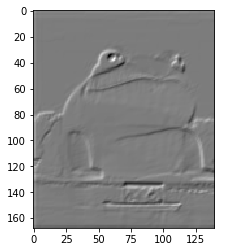
\includegraphics[width=\linewidth]{images/poly_nr_lin.png}
    \caption{Local Poly Reg Lin(true)}
  \end{subfigure}
  \begin{subfigure}[b]{0.24\linewidth}
    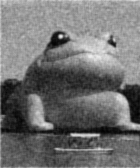
\includegraphics[width=\linewidth]{images/poly_nr_true.png}
    \caption{Local Poly Reg Cons(h=1)}
  \end{subfigure}
  \begin{subfigure}[b]{0.24\linewidth}
    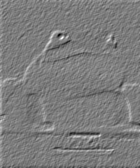
\includegraphics[width=\linewidth]{images/poly_nr_lin_true.png}
    \caption{Local Poly Reg Lin(h=1)}
  \end{subfigure}
  \caption{Local polynomial regression results}
  \label{fig:local_poly}
\end{figure}

\begin{figure}[htb]
  \centering
  \begin{subfigure}[b]{0.24\linewidth}
    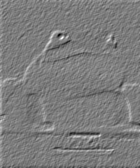
\includegraphics[width=\linewidth]{images/edge_1.png}
    \caption{LPR linear term coef}
  \end{subfigure}
  \begin{subfigure}[b]{0.24\linewidth}
    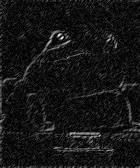
\includegraphics[width=\linewidth]{images/edge_2.png}
    \caption{LPR linear term abs coef}
  \end{subfigure}
  \begin{subfigure}[b]{0.24\linewidth}
    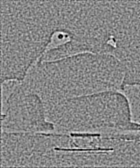
\includegraphics[width=\linewidth]{images/edge_3.png}
    \caption{LoG($\sigma=1$)}
  \end{subfigure}
  \begin{subfigure}[b]{0.24\linewidth}
    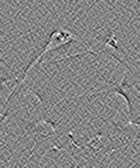
\includegraphics[width=\linewidth]{images/edge_4.png}
    \caption{Sobel}
  \end{subfigure}
  \caption{How linear term in LPR can be explained as edge detection}
  \label{fig:edge}
\end{figure}



\subsection{Cross validation for smoothing}

%Since the image usually include too many data point. Using local property appearing in image processing 
%will be helpful when evaluate the leave-one-out cross-validation score.

Since here we have actually the true function $r(i,j)$, the vanilla risk:

$$
R(h) = E \left( \frac{1}{n}\sum_{i=1}^n(\hat{r}_n(x_i)-r(x_i))^2 \right)
$$

for given $h,\sigma$ (the randomness of $\hat{r}_n(x_i)$ is subject to $\sigma$ parameter of noise term $\epsilon$) 
can be approximated by Monte Calor simulation:

$$
R(h) \approx \frac{1}{T} \sum_{t=1}^T \frac{1}{n}\sum_{i=1}^n(\hat{r}_n(x_i)-r(x_i))^2
$$

The $T$ is number of simulation, here $T=200$ is used. See Fig~\ref{fig:crossvalidation_mc}
\footnote{Note Julia treat gray image as $[0,1]$ float number instead of $[0,255]$ in Python. Following content is based on Julia,
so a $\sigma=25$ noise in range $[0,255]$ for MatLab/Python is equivalence to $0.098$ in range $[0,1]$ for Julia.}
 for result of simulation with mean with $3\sigma$ ribbon. 
It's obvious that the optimal may be located in $h \approx 0.75$ .

\begin{figure}[htb]
  \centering
  \begin{subfigure}[b]{0.49\linewidth}
    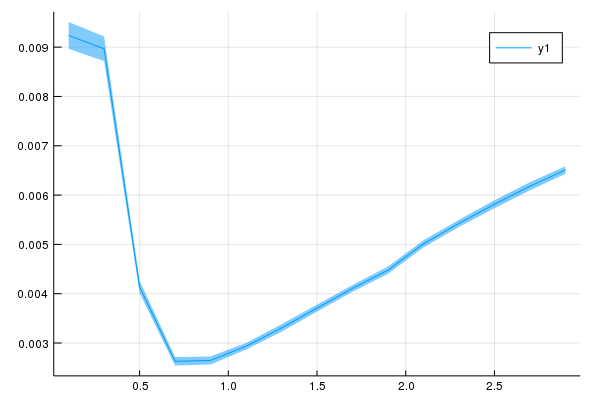
\includegraphics[width=\linewidth]{images/crossvalidation1.png}
    \caption{Monte Carlo $R(h)$ for the true image}
    \label{fig:crossvalidation_mc}
  \end{subfigure}
  \begin{subfigure}[b]{0.49\linewidth}
    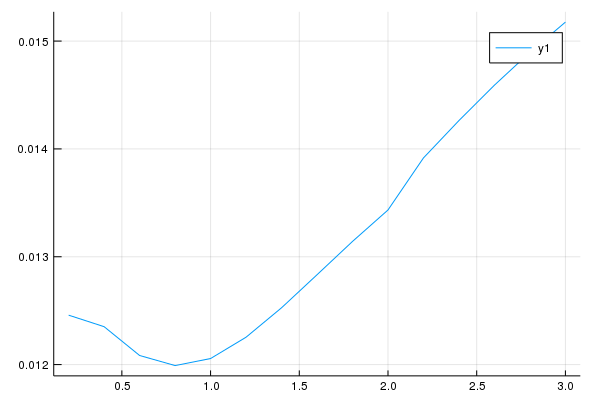
\includegraphics[width=\linewidth]{images/crossvalidation2.png}
    \caption{CV for a given noised image}
    \label{fig:crossvalidation_cv}
  \end{subfigure}
  \caption{Cross Validation}
  \label{fig:crossvalidation}
\end{figure}

Of course usually we don't have true function $r(x_i)$, so we want a sample-based method, 
that is the leave-one-out cross validation score which can be employed to show a guideline to choose optimal bandwidth $h$
when true function is not observed.

Fortunately, the LOOCV is equivalence to remove the center of the kernel used in filtering, so that we can simplify this to 
convolution which can be effectively computed by software.

The vanilla equation:

$$
CV = \hat{R}(h)=\frac{1}{n}\sum_{i=1}^n (Y_i-\hat{r}_{-i}(x_i))^2
$$

is equivalence to following change of kernel of convolution in gaussian kernel regression, see Fig~\ref{fig:gaussian_kernel}. 
The result can seen in Fig~\ref{fig:crossvalidation_cv}.

The Equation(5.36) in \cite{wasserman2006all} define the generalized cross validation:

$$
GCV = \frac{1}{n}\sum_{i=1}^n \left(\frac{Y_i-\hat{r}_n(x_i)}{1-\nu/n}\right)^2
$$

Where $\nu = \sum_{i=1}^n \mathbf{L}_{ii}$. Since the kernel used in gaussian kernel regression is homogeneous(i.e. it always take $0.1621$
shown in \ref{fig:gaussian_kernel} when $h=1$.). Therefore $L_{ii} = \nu/n$, thus the GCV take same value as CV take. 

\begin{figure}[htb]
  \centering
  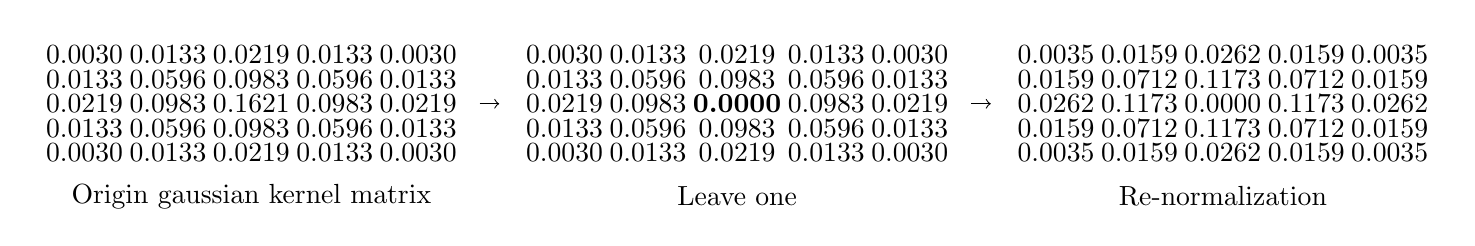
\begin{tikzpicture}
    \matrix [matrix of nodes,row sep=-1ex, column sep=-1ex, anchor=west] (kernel_ori) at (0.0, 0.0)
    {
        0.0030 & 0.0133 & 0.0219 & 0.0133 & 0.0030 \\
        0.0133 & 0.0596 & 0.0983 & 0.0596 & 0.0133 \\
        0.0219 & 0.0983 & 0.1621 & 0.0983 & 0.0219 \\
        0.0133 & 0.0596 & 0.0983 & 0.0596 & 0.0133 \\
        0.0030 & 0.0133 & 0.0219 & 0.0133 & 0.0030 \\    };
    
        \matrix [matrix of nodes,row sep=-1ex, column sep=-1ex, anchor=west] (kernel_tra) at ([shift={(0.4, 0.00)}]kernel_ori.east)
    {
        0.0030 & 0.0133 & 0.0219 & 0.0133 & 0.0030 \\
        0.0133 & 0.0596 & 0.0983 & 0.0596 & 0.0133 \\
        0.0219 & 0.0983 & \bf{0.0000} & 0.0983 & 0.0219 \\
        0.0133 & 0.0596 & 0.0983 & 0.0596 & 0.0133 \\
        0.0030 & 0.0133 & 0.0219 & 0.0133 & 0.0030 \\    };

        \matrix [matrix of nodes,row sep=-1ex, column sep=-1ex, anchor=west] (kernel_tra2) at ([shift={(0.4, 0.00)}]kernel_tra.east)
    {
        0.0035 & 0.0159 & 0.0262 & 0.0159 & 0.0035 \\
        0.0159 & 0.0712 & 0.1173 & 0.0712 & 0.0159 \\
        0.0262 & 0.1173 & 0.0000 & 0.1173 & 0.0262 \\
        0.0159 & 0.0712 & 0.1173 & 0.0712 & 0.0159 \\
        0.0035 & 0.0159 & 0.0262 & 0.0159 & 0.0035 \\
    };



    \draw [->] ([shift={(0.05, -0.00)}]kernel_ori.east) to [out=0, in=180] ([shift={(-0.1, 0.00)}]kernel_tra.west);
    \draw [->] ([shift={(0.05, -0.00)}]kernel_tra.east) to [out=0, in=180] ([shift={(-0.1, 0.00)}]kernel_tra2.west);

    \node at ([shift={(0.0, -0.2)}]kernel_ori.south) {Origin gaussian kernel matrix};
    \node at ([shift={(0.0, -0.2)}]kernel_tra.south) {Leave one};
    \node at ([shift={(0.0, -0.2)}]kernel_tra2.south) {Re-normalization};

\end{tikzpicture}

  \caption{Gaussian kernel used in Leave-one-out cross validation}
  \label{fig:gaussian_kernel}
\end{figure}


\subsection{Variance estimation introduced by smoothing}

In fact, the image is polluted by some i.i.d noise terms $\epsilon_i \sim N(0,\sigma^2)$ where hold a constant $\sigma$ for every index $i$.
so that, following \cite{wasserman2006all} Theorem 5.85, we can estimate it by following equation:

$$
\hat{\sigma}^2=\frac{\sum_{i=1}^n (Y_i-\hat{r}(x+i))^2}{n-2\nu+\tilde{\nu}}
$$

where

$$
\nu = \mathrm{tr}(\mathbf{L}), \quad 
\tilde{\nu}=\mathrm{tr}(\mathbf{L}^T\mathbf{L})=\sum_{i=1}^n||l(x_i)||^2
$$

In our setting, let $K$ denote the kernel matrix
\footnote{The $K$ can be encoded as a sparse 23520 dimension vector $l_i$ which have 25 non-zero value while all other value are zero to match
the notation used in the textbook, but those tedious transform are omitted for briefly.}
such as the one shown in Fig~\ref{fig:gaussian_kernel} leftmost.
$n = 168 \times 140 = 23520$,$\nu = n \times s \times K[0,0]$,
$\tilde{\nu} = \sum_{i=-2}^2\sum_{j=-2}^2 K[i,j]^2$. 
Set $\sigma=50$(In Julia it's $\sigma=0.098$), 
the simulation distribution of $\hat{\sigma}^2$ can be seen in Fig~\ref{fig:std_est}. 
The interesting thing is that all of them fail to cover true point $0.098$, when $h$ become larger,
the bias is even worsen, though the range of $(h=0.2)$, $[0.1000,0.1024]$ almost capture it.
It's not that surprise considering the consistency condition of estimator, 
$\nu=o(n),\tilde{\nu}=o(n)$ which is not satisfied in this case.

\begin{figure}[htb]
  \centering
  \begin{subfigure}[b]{0.24\linewidth}
    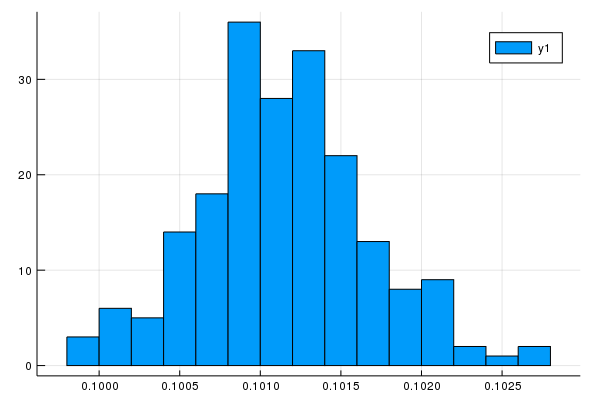
\includegraphics[width=\linewidth]{images/std_est_1.png}
    \caption{Dist of $\hat{\sigma}^2$ ($h=0.2$)}
  \end{subfigure}
  \begin{subfigure}[b]{0.24\linewidth}
    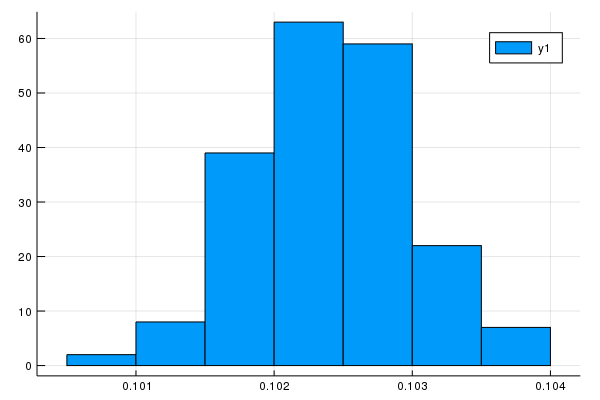
\includegraphics[width=\linewidth]{images/std_est_2.png}
    \caption{Dist of $\hat{\sigma}^2$ ($h=0.5$)}
  \end{subfigure}
  \begin{subfigure}[b]{0.24\linewidth}
    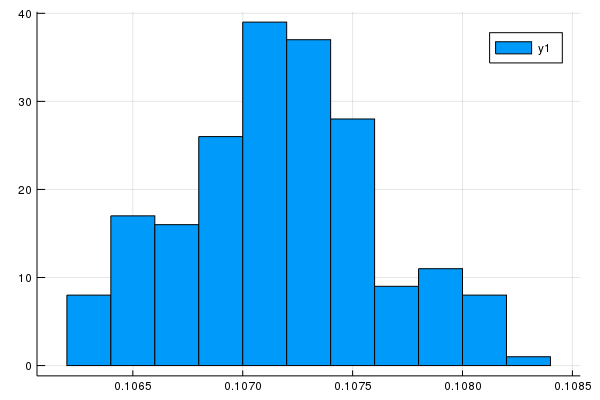
\includegraphics[width=\linewidth]{images/std_est_3.png}
    \caption{Dist of $\hat{\sigma}^2$ ($h=1.0$)}
  \end{subfigure}
  \begin{subfigure}[b]{0.24\linewidth}
    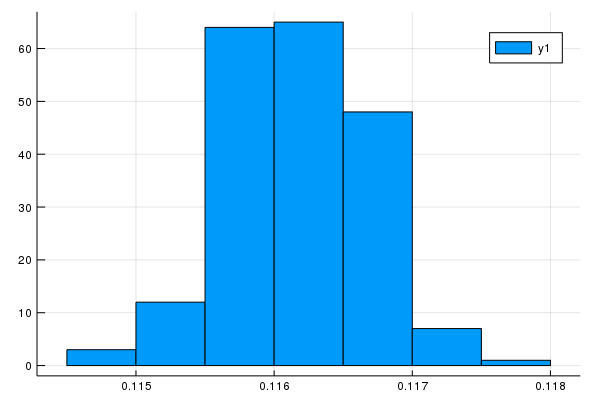
\includegraphics[width=\linewidth]{images/std_est_4.png}
    \caption{Dist of $\hat{\sigma}^2$ ($h=2.0$)}
  \end{subfigure}
  \caption{simulation distribution of $\hat{\sigma}^2$(samples = 200)}
  \label{fig:std_est}
\end{figure}

\section{Density estimation and threshold segmentation}

\label{segmentation}

Due to the property of linear combination of Eq~\ref{eq:rgb_to_gray}. Splitting the image from RGB to three channel histogram is more useful
compared to using gray histogram directly. For example, the result of toad is shown in Fig~\ref{fig:hist_g_rgb}.

\begin{figure}[htb]
  \centering
  \begin{subfigure}[b]{0.24\linewidth}
    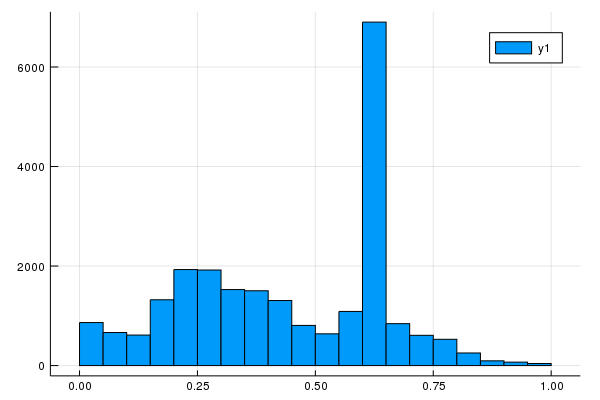
\includegraphics[width=\linewidth]{images/hist_gray.png}
    \caption{Hist of gray}
  \end{subfigure}
  \begin{subfigure}[b]{0.24\linewidth}
    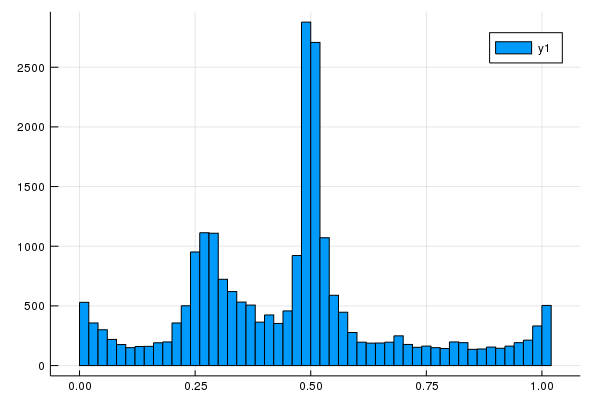
\includegraphics[width=\linewidth]{images/hist_r.png}
    \caption{Hist of red}
  \end{subfigure}
  \begin{subfigure}[b]{0.24\linewidth}
    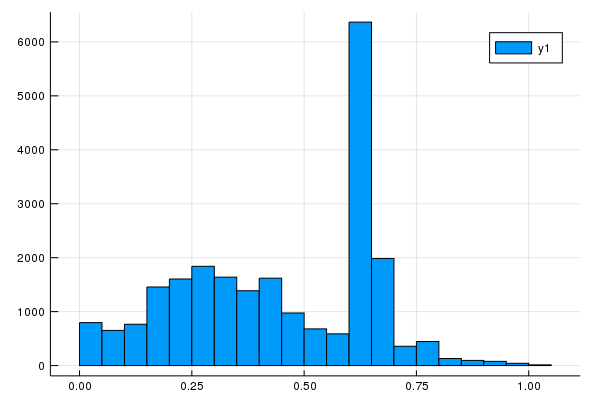
\includegraphics[width=\linewidth]{images/hist_g.png}
    \caption{Hist of green}
  \end{subfigure}
  \begin{subfigure}[b]{0.24\linewidth}
    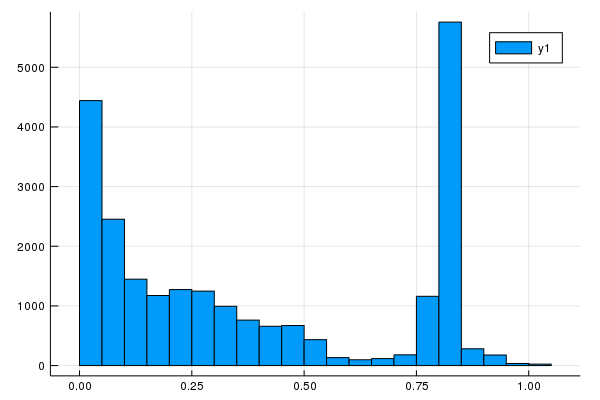
\includegraphics[width=\linewidth]{images/hist_b.png}
    \caption{Hist of blue}
  \end{subfigure}
  \caption{Splitting three channel histogram}
  \label{fig:hist_g_rgb}
\end{figure}

Histogram is subject to bins, we want to look for a smoothed version of histogram t
hat can either corporate "bandwidth" information and keep its continues property(resolution). 
A choice is Kernel Density Estimation(KDE). Eq(6.26) in \cite{wasserman2006all} show:

$$
\hat{f} = \frac{1}{n} \sum_{i=1}^n \frac{1}{h} K\left( \frac{x-X_i}{h} \right)
$$

I choose Gaussian Kernel, $K(x)=\frac{1}{\sqrt{2\pi}}e^{-x^2/2}$ with $h=0.3$, 
the result is shown in Fig~\ref{fig:kde}.

\begin{figure}[htb]
  \centering
  \begin{subfigure}[b]{0.24\linewidth}
    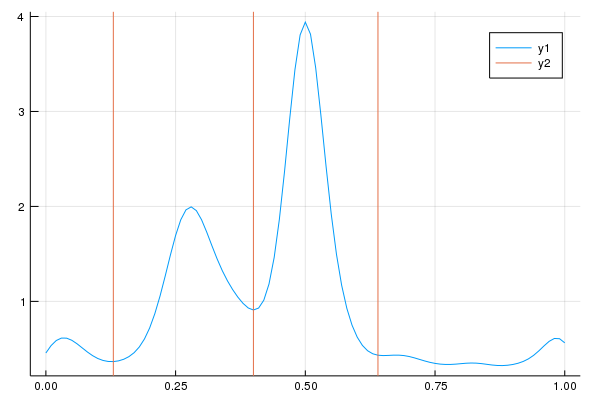
\includegraphics[width=\linewidth]{images/kde_r.png}
    \caption{KDE of red}
  \end{subfigure}
  \begin{subfigure}[b]{0.24\linewidth}
    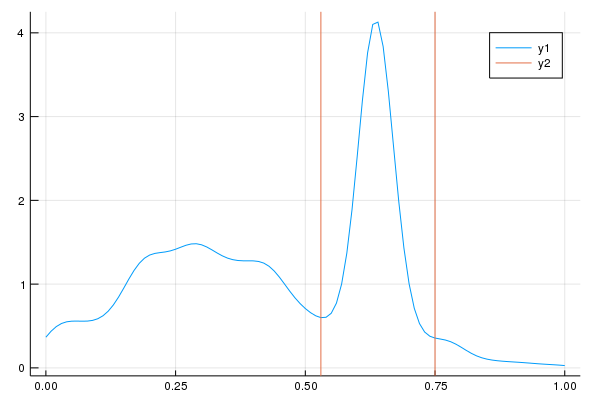
\includegraphics[width=\linewidth]{images/kde_g.png}
    \caption{KDE of green}
  \end{subfigure}
  \begin{subfigure}[b]{0.24\linewidth}
    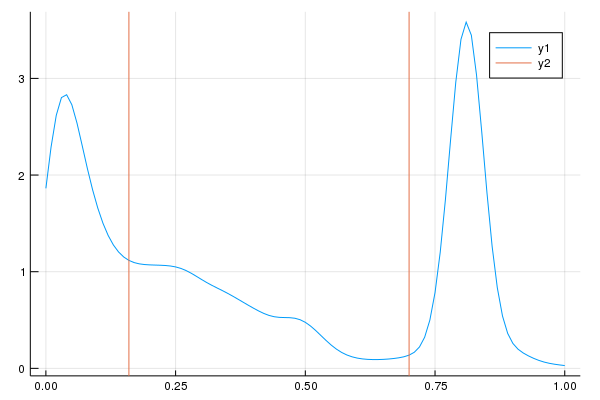
\includegraphics[width=\linewidth]{images/kde_b.png}
    \caption{KDE of blue}
  \end{subfigure}
  \begin{subfigure}[b]{0.24\linewidth}
    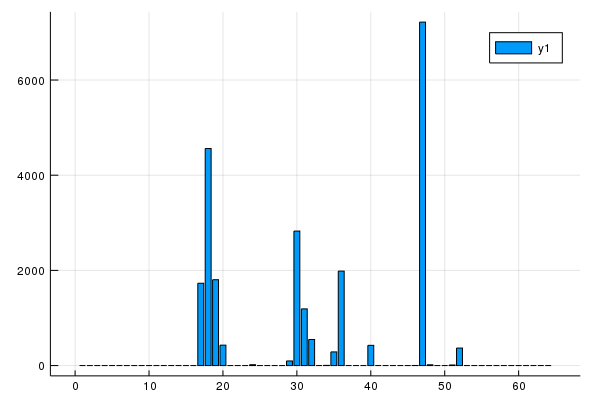
\includegraphics[width=\linewidth]{images/kde_code.png}
    \caption{Encoding of KDE}
  \end{subfigure}
  \caption{KDE and threshold encoding}
  \label{fig:kde}
\end{figure}

Some vertical lines are drawn to indicate some "components" behind in the image. 
We can assume that some region of the image space is segmented firstly (latent variables) 
and draw centering color and correlated noise(i.e. MRF) on it. 
To infer the latent class label in image region,
we can use clustering such as k-means with a distance measure such as distance of pixel and color. 
But here, one observe the KDE of image,
manually or automatically choose some cutoff points(Here points is chosen manually, 
but taking minimum value of KDE numerically can be employed.). 
So in principle we can get $4\times 3\times 3=36$ components, 
but since RGB is correlated in intensity(say, more red value imply more green and blue value as well.), 
the number of valid components is only $18$ as shown in \ref{fig:kde}.
Those components can be split into a image, as shown in \ref{fig:splitting}. 
The processing result of it is called segmentation, a classic field in image processing. 
Anyway the method using KDE is not that useful compared to modern method using CNN \cite{long2015fully} or 
even early method using MRF\cite{panjwani1995markov}. 

\begin{figure}[htb]
  \centering
  \begin{subfigure}[b]{0.24\linewidth}
    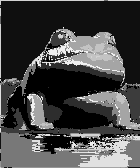
\includegraphics[width=\linewidth]{images/toad_split.png}
    \caption{Weird toad splitting}
  \end{subfigure}
  \begin{subfigure}[b]{0.24\linewidth}
    
\includegraphics[width=\linewidth]{images/toad_split_air.png}
    \caption{Splitting of air}
  \end{subfigure}
  \begin{subfigure}[b]{0.24\linewidth}
    
\includegraphics[width=\linewidth]{images/toad_split_center.png}
    \caption{Splitting of back}
  \end{subfigure}
  \begin{subfigure}[b]{0.24\linewidth}
    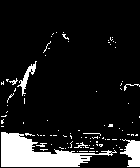
\includegraphics[width=\linewidth]{images/toad_split_water.png}
    \caption{Splitting of part of water}
  \end{subfigure}
  \caption{KDE and segmentation}
  \label{fig:splitting}
\end{figure}

\section{Converting Density Estimation into Regression to suppress minimum value made by noise}

Automatically detecting cutoff points through searching on local minimum is subject to some factors. 
If there is a minimum point, but with very tiny curvature, is it a true minimum point or made by random noise? 
It may occur more usually when $h$ is not "enough".
For example, Fig~\ref{fig:DS_REG} show the KDE of red and blue channels when $h=0.2$ compared to previous $h=0.3$.
We can impose a confidence interval to it to determine. 
It require technique in \cite{wasserman2006all} section 6.6.

Firstly divide the interval [0,1] (Julia treat intensity as number in $[0,1]$ exactly) into $k=100$ bins, 
which center is denoted by $X_1,\dots,X_k$. Let $N_j$ be the number of observations in bin $j$. Define

$$
Y_j = \sqrt{\frac{k}{n}} \times \sqrt{N_j+\frac{1}{4}}
$$

So now we have a standard regression problem for data $(X_j,Y_j),j=1,\dots,k$.
Gaussian kernel regression with $h=1$ is used to solve it, the result can shown in Fig~\ref{fig:DS_REG}.
The wide confidence band around those suspicion minimum points indicate that they're fake ones.
 
\begin{figure}[htb]
  \centering
  \begin{subfigure}[b]{0.24\linewidth}
    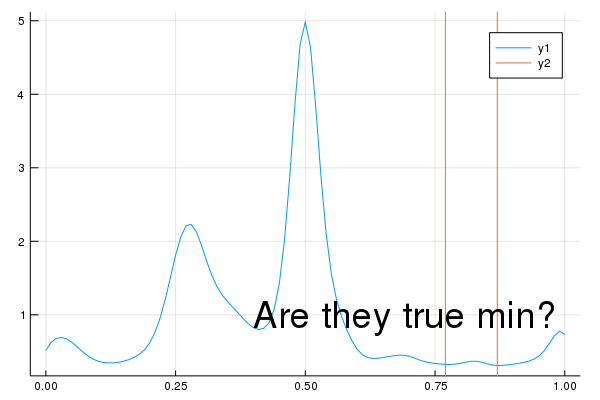
\includegraphics[width=\linewidth]{images/fake_min_r.png}
    \caption{KDE of red ($h=0.2$)}
  \end{subfigure}
  \begin{subfigure}[b]{0.24\linewidth}
    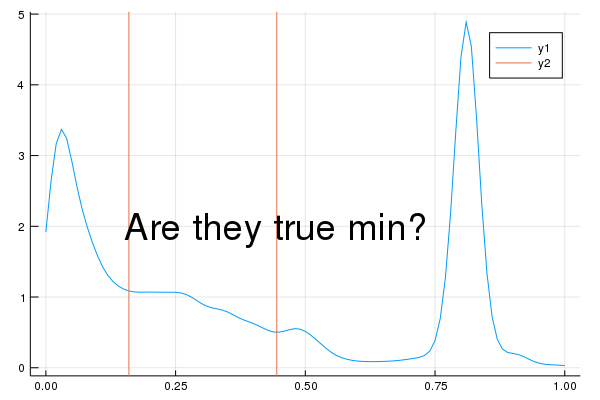
\includegraphics[width=\linewidth]{images/fake_min_b.png}
    \caption{KDE of blue ($h=0.2$)}
  \end{subfigure}
  \begin{subfigure}[b]{0.24\linewidth}
    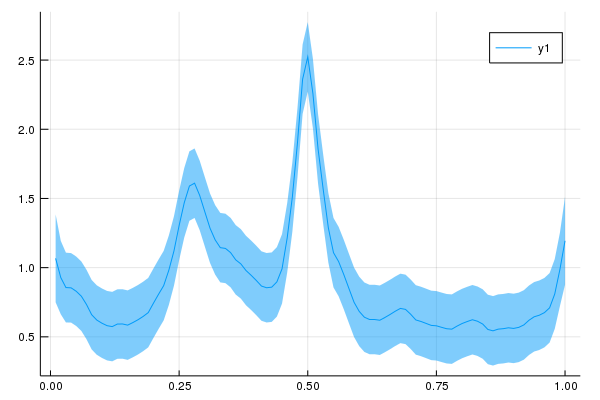
\includegraphics[width=\linewidth]{images/kde_reg_r.png}
    \caption{Red DS by KR($h=1.0$) with 3$\sigma$ range}
  \end{subfigure}
  \begin{subfigure}[b]{0.24\linewidth}
    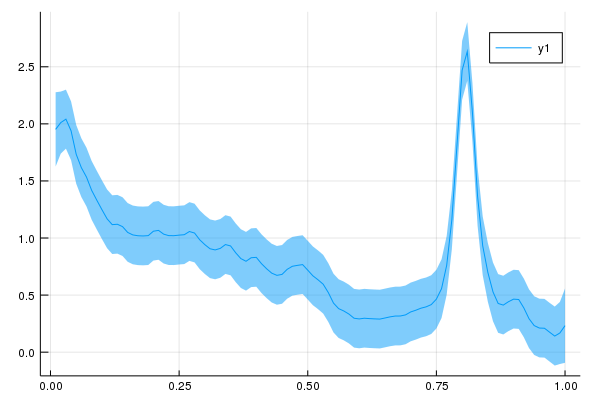
\includegraphics[width=\linewidth]{images/kde_reg_b.png}
    \caption{Blue DS by KR($h=1.0$) with 3$\sigma$ range}
  \end{subfigure}
  \caption{Some possible fake minimum points and suppressing}
  \label{fig:DS_REG}
\end{figure}


\section{Bootstrap and confidence of feature detecting}

\cite{ghorbel1994bootstrap} propose a interesting idea to use bootstrap in invariant feature for image processing.
I will extent it for matching.

\subsection{Invariant feature: Hu moments}

A image or patch of image can be summarized by some statistic, such as intensity histogram shown above. If we impose some constraints
on those statistic, for example, they should be invariant to translate, scale, rotation transform. The valid choose of those statistic
seems narrow, a excellent result is obtained by \cite{hu1962visual}, called Hu moments, which is defined by:

\begin{align}
  \begin{split}
    M_{ij} &= \sum_x \sum_y x^i y^i I(x,y) \\
    \bar{x} &= \frac{M_{10}}{M_{00}} \\
    \bar{y} &= \frac{M_{01}}{M_{00}} \\
    \mu_{ij} &= \sum_x \sum_y (x-\bar{x})^i(y-\bar{y})^j I(x,y)\\
    \eta_{ij} &= \frac{\mu_{i,j}}{\mu_{00}^{(i+j)/2+1}} \\
    h_0 &= \eta_{20}+\eta_{02} \\
    h_1 &= (\eta_{20} - \eta_{02})^2 + 4\eta_{11}^2 \\
    h_2 &= (\eta_{30} + \eta_{12})^2 + (\eta_{21}+\eta_{03})^2 \\
    h_3 &= (\eta_{30}-3\eta_{12})(\eta_{30}+\eta_{12})[(\eta_{30}+\eta_{12})^2-3(2\eta_{21}+\eta_{03})^2] + (3\eta_{21}-\eta_{03})[3(\eta_{30}+\eta_{12})^2-(\eta_{21}+\eta_{03})^2] \\
  \end{split} 
  \label{eq:mu_moment}
\end{align}

The full definition of Hu moments include $h_5,h_6$, but here I don't use them due to
numerical problem. 

Anyway, Mu moments map a $M \times N$ image into a $R^4$ vector, usually we take $\log(.)$ to normalize them.

\subsection{Integrating bootstrap}

Given any feature, we can compute distance between two images using their corresponding vector given by the features. But how can we know
they're \textit{significant}? Say we observe a big distance and a small distance, it's not determined whether the difference of first one is 
big than second one since we don't know the volatility in the two "testing". Bootstrap provide a nice way to estimate the volatility/variance
of those distance.

Section 3.2 in \cite{wasserman2006all} defined the Bootstrap Variance Estimation:

$$
v_{boot} = \frac{1}{B} \sum_{b=1}^B \left( T^*_{n,b} - \frac{1}{B}\sum_{r=1}^B T^*_{n,r} \right)^2
$$

Where $T_n^*=g(X_1^*,\dots,X_n^*)$ is some statistics and samples $X_1^*,\dots,X_n^* \sim \hat{F}_n$ is sampled from given data $X_1^*,\dots,X_n^*$.

We see image $x_{ij}$ as list of data $(i,j,I(i,j))$(Eq~\ref{eq:mu_moment} is converted to corresponding form), and thus we can sample them as usual,
and let $H(x_{ij})$ be Hu moment, $D(x,y)=||H(x_{ij}) - H(y_{ij})||^2$ be "distance" between two images/patches, $x_t^*(i,j)$ be a re-sampled
image data(now, generally it can not construct a valid image) from given image $x(i,j)$, $D(x_t^*,y_t^*)$ be distance of two re-sampled images. Thus we can define $v_{boot}^I$ as:

$$
v_{boot}^I = \frac{1}{B}\sum_{b=1}^B \left( D(x_b^*,y_b^*) - \frac{1}{B} \sum_{r=1}^B D(x_r^*,y_r^*) \right)^2
$$

Here $B=100$, dividing the image into $3 \times 3$ patches, the result can be shown in Fig~\ref{fig:square33}. 
$D(x,y)$ is computed for every neighboring pair of pixels. The number after $\pm$ is $\sqrt{v_{boot}}$. It can be show that
the difference of first and second row is significantly big than difference of second and third row. In more dense grid,
we may extract a rough segmentation cut from that grid.

\begin{figure}[htb]
  \centering
  \begin{tikzpicture}
    \node[inner sep=0pt] (toad_1_1) at (0,0)
    {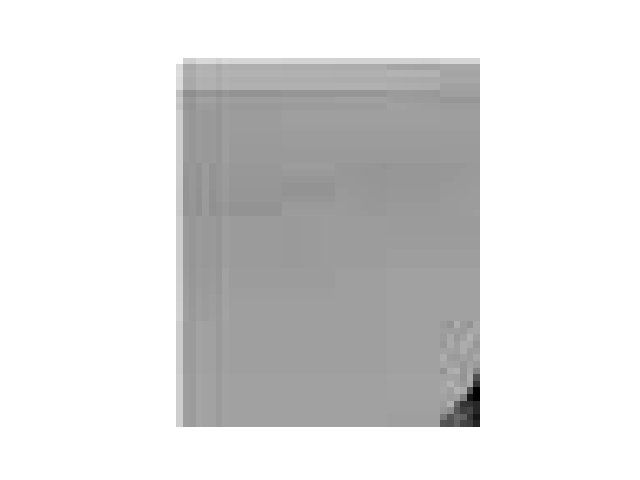
\includegraphics[width=.3\textwidth]{images/toad_1_1.png}};
    \node[inner sep=0pt] (toad_2_1) at ([shift={(0.0, -1.5)}]toad_1_1.south)
    {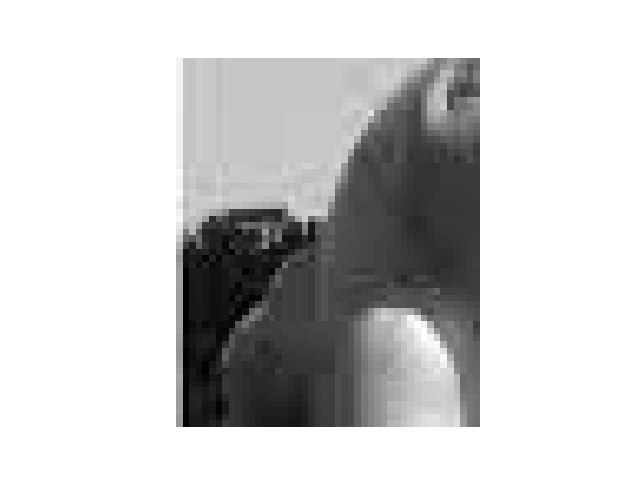
\includegraphics[width=.3\textwidth]{images/toad_2_1.png}};
    \node[inner sep=0pt] (toad_3_1) at ([shift={(0.0, -1.5)}]toad_2_1.south)
    {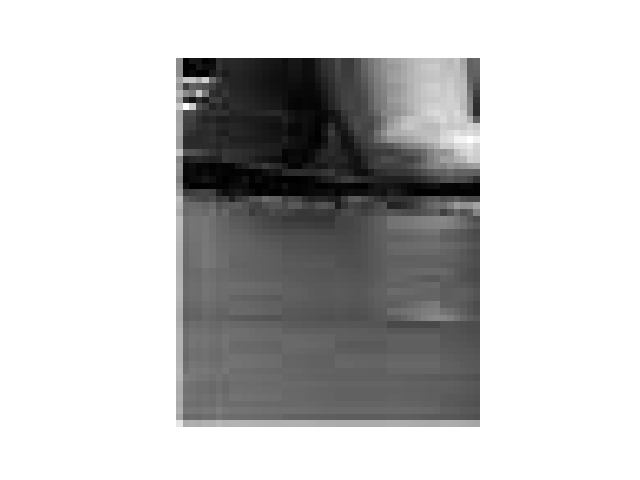
\includegraphics[width=.3\textwidth]{images/toad_3_1.png}};
    \node[inner sep=0pt] (toad_1_2) at ([shift={(2.5, 0.0)}]toad_1_1.east)
    {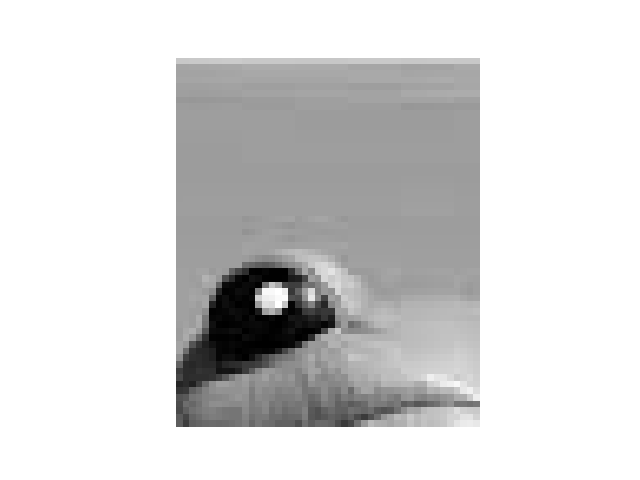
\includegraphics[width=.3\textwidth]{images/toad_1_2.png}};
    \node[inner sep=0pt] (toad_2_2) at ([shift={(0.0, -1.5)}]toad_1_2.south)
    {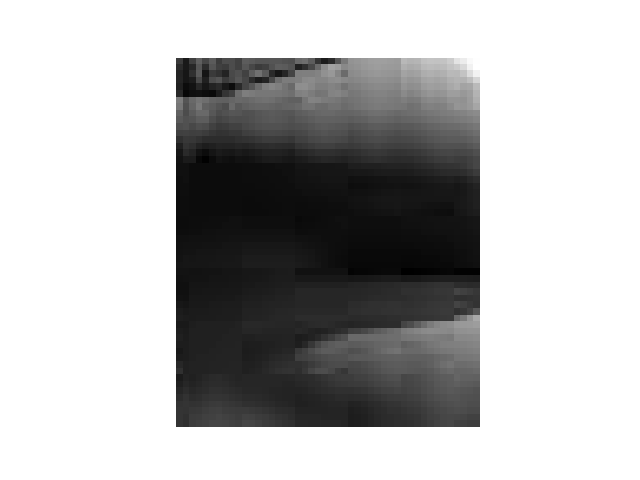
\includegraphics[width=.3\textwidth]{images/toad_2_2.png}};
    \node[inner sep=0pt] (toad_3_2) at ([shift={(0.0, -1.5)}]toad_2_2.south)
    {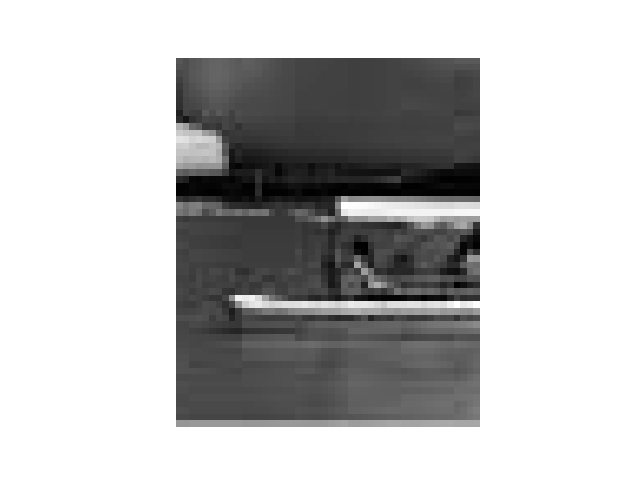
\includegraphics[width=.3\textwidth]{images/toad_3_2.png}};
    \node[inner sep=0pt] (toad_1_3) at ([shift={(2.5, 0.0)}]toad_1_2.east)
    {\includegraphics[width=.3\textwidth]{images/toad_1_3.png}};
    \node[inner sep=0pt] (toad_2_3) at ([shift={(0.0, -1.5)}]toad_1_3.south)
    {\includegraphics[width=.3\textwidth]{images/toad_2_3.png}};
    \node[inner sep=0pt] (toad_3_3) at ([shift={(0.0, -1.5)}]toad_2_3.south)
    {\includegraphics[width=.3\textwidth]{images/toad_3_3.png}};

    \draw [-] (toad_1_1.east) -- (toad_1_2.west) node [midway, below] {$ 24.988 \pm 22.369 $};
    \draw [-] (toad_1_1.south) -- (toad_2_1.north) node [midway, left] {$ 117.053 \pm 42.209 $};
    \draw [-] (toad_1_2.east) -- (toad_1_3.west) node [midway, below] {$ 16.502 \pm 11.726 $};
    \draw [-] (toad_1_2.south) -- (toad_2_2.north) node [midway, left] {$ 14.012 \pm 3.556 $};
    \draw [-] (toad_1_3.south) -- (toad_2_3.north) node [midway, left] {$ 44.610 \pm 17.570 $};
    \draw [-] (toad_2_1.east) -- (toad_2_2.west) node [midway, below] {$ 8.931 \pm 3.148 $};
    \draw [-] (toad_2_1.south) -- (toad_3_1.north) node [midway, left] {$ 2.160 \pm 0.927 $};
    \draw [-] (toad_2_2.east) -- (toad_2_3.west) node [midway, below] {$ 3.937 \pm 2.340 $};
    \draw [-] (toad_2_2.south) -- (toad_3_2.north) node [midway, left] {$ 5.036 \pm 7.379 $};
    \draw [-] (toad_2_3.south) -- (toad_3_3.north) node [midway, left] {$ 1.577 \pm 1.423 $};
    \draw [-] (toad_3_1.east) -- (toad_3_2.west) node [midway, below] {$ 10.723 \pm 10.646 $};
    \draw [-] (toad_3_2.east) -- (toad_3_3.west) node [midway, below] {$ 6.596 \pm 7.907 $};

    %\draw[help lines] (0,0) grid (10,-10);
\end{tikzpicture}

  \caption{$3 \times 3$ Squares of patches of toad and their neighbor distance using Hu moment with bootstrap $\sqrt{v_{boot}}$}
  \label{fig:square33}
\end{figure}

\section{Conclusion}

In this work, noise removal problem using non-parametric regression and their relationship to methods in traditional image processing 
is discovered and illustrated. Kernel regression is fast and effective, while local polynomial is too costly and fail to get significant
improvement compared to kernel regression. How to use cross validation of theory, leave-one-out fashion and GCV are surveyed, it show
a idea curve which is similar to one listed in \cite{wasserman2006all}. Variance estimation using smoothing get almost exact result. Density estimation
technique such as histogram and kernel density is used to build a rough segmentation, the variance of density estimation introduced by
converting problem to regression is used to suppress fake minimum therefore may help to automatically cutting point detection. Finally, 
how to incorporate the variance information provided by bootstrap into Hu moment to evaluate their difference is shown.

Though those are poor enough methods compared to modern approaches. The interdisciplinary relationship is still interesting. 


\bibliographystyle{unsrt}  
\bibliography{references}  %%% Remove comment to use the external .bib file (using bibtex).
%%% and comment out the ``the bibliography'' section.

\appendix

\section{Appendix: Part of Julia code used in experiment}

%\subsection{Kernel regression}

\subsection{Local polynomial}

\begin{lstlisting}
ii = [i for i=1:size(toad_noised,1),j=1:size(toad_noised,2)] 
jj = [j for i=1:size(toad_noised,1),j=1:size(toad_noised,2)] 
iijj = cat(reshape(ii,1,size(ii,1),size(ii,2)),
  reshape(jj,1,size(jj,1),size(jj,2)),dims=1)
IJ = reshape(iijj, 2, size(iijj,2)*size(iijj,3))

dis = Normal()
K = x->pdf(dis,x)

mat = zeros(3, size(toad_noised,1), size(toad_noised,2))

for i=1:size(toad_noised,1)
    for j=1:size(toad_noised,2)
        ij = [i;j]
        Wx = K.(sum(abs.(ij .- IJ),dims=1))
        _X = sum(ij .- IJ, dims=1)
        X = cat(1, _X, dims=1)

        l = inv((X .* Wx) * X') * (X .* Wx)
        a = l * Y'

        mat[1,i,j] = a[1,1]
        mat[2,i,j] = a[2,1]
        mat[3,i,j] = sum(l.^2)
    end
end
\end{lstlisting}

\subsection{Cross validation}

\subsubsection{Monte Carlo}

\begin{lstlisting}
sigma_noise = 25
simga_imfilter_range = 0.1:0.2:3
T = 200

sigma_loss_list = zeros(length(simga_imfilter_range))
sigma_loss_std_list = zeros(length(simga_imfilter_range))

for simga_imfilter_idx=1:length(simga_imfilter_range)
    simga_imfilter = simga_imfilter_range[simga_imfilter_idx]
    loss_list = zeros(T)
    for t=1:T
        toad_noised = clamp.(convert(Array{Float64}, 
          toad + rand(Normal(0,sigma_noise/255), size(toad))), 0.0, 1.0)
        toad_filtered = imfilter(Gray.(toad_noised), 
          Kernel.gaussian(simga_imfilter))
        loss_list[t] = mean((toad_filtered - toad).^2)
    end
    sigma_loss_list[simga_imfilter_idx] = mean(loss_list)
    sigma_loss_std_list[simga_imfilter_idx] = std(loss_list)
end
\end{lstlisting}

\subsubsection{CV/GCV}

\begin{lstlisting}
sigma_noise = 25
simga_imfilter_range = 0.2:0.2:3
T = 200

sigma_loss_list = zeros(length(simga_imfilter_range))
sigma_loss_std_list = zeros(length(simga_imfilter_range))

for simga_imfilter_idx=1:length(simga_imfilter_range)
    simga_imfilter = simga_imfilter_range[simga_imfilter_idx]
    
    K = Kernel.gaussian(simga_imfilter)
    K[0,0]=0
    K = K./sum(K)
    toad_filtered = imfilter(Gray.(toad_noised), K)
    
    #sigma_loss_list[simga_imfilter_idx] = mean((toad_filtered - toad).^2)
    sigma_loss_list[simga_imfilter_idx] = mean((toad_filtered - toad_noised).^2)
end

\end{lstlisting}

\subsection{Kernel density estimation}

\begin{lstlisting}
h=0.1
dis = Normal()
K = x->pdf(dis,x)
diff = (reshape(x,size(x,1),1) .- reshape(X,1,size(X,1))) ./ h
f = sum(K.(diff), dims=2) / size(X,1) / h
\end{lstlisting}

\subsection{Density estimation using kernel regression}

\begin{lstlisting}
X = vec(convert(Array{Float64}, toad_r))

_size = 100
X_seg=1:1:100
N_seg = zeros(Int,_size)
for Xi in X
    #println(Int(trunc(Xi*(_size-1))))
    N_seg[Int(trunc(Xi*(_size-1)))+1] += 1
end

Y_seg = sqrt(100/size(X)[1]) .* sqrt.(N_seg .+ 0.25);

h = 1.0

L_n = K.((reshape(X_seg, size(X_seg,1),1) .- 
  reshape(X_seg, 1, size(X_seg,1)))./h)

L = L_n ./ reshape(sum(L_n,dims=2),size(L_n,1),1)

r = L * Y_seg

\end{lstlisting}

\subsection{Bootstrap and features}

\begin{lstlisting}

function hu_M(arr,i,j)
  # arr: [[ii_1,jj_1,I_1],[ii_2,jj_2,I_2],...]
  return sum(arr[:,1].^i .* arr[:,2].^j .* arr[:,3])
end

function hu_mu(arr,i,j)
  M00 = hu_M(arr, 0, 0)
  M10 = hu_M(arr, 1, 0)
  M01 = hu_M(arr, 0, 1)
  
  x_bar = M10/M00
  y_bar = M01/M00
  
  return sum((arr[:,1].-x_bar).^i .* (arr[:,2].-y_bar).^j .* arr[:,3])
end

function hu_eta(arr, i, j)
  mu00 = hu_mu(arr, 0, 0)
  return hu_mu(arr, i, j)/mu00^((i+j)/2+1)
end

function hu_hu(arr)
  eta20 = hu_eta(arr, 2, 0)
  eta02 = hu_eta(arr, 0, 2)
  eta11 = hu_eta(arr, 1, 1)
  eta12 = hu_eta(arr, 1, 2)
  eta21 = hu_eta(arr, 2, 1)
  eta30 = hu_eta(arr, 3, 0)
  eta03 = hu_eta(arr, 0, 3)
  
  mu03 = hu_mu(arr, 0, 3)
  
  hu1 = eta20+eta02
  hu2 = (eta20-eta02)^2 + 4*eta11^2
  #hu3 = (eta30-3*eta12)^2 + (3*eta21-mu03)^2
  #hu4 = (eta30+eta12)^2 + (eta21+mu03)^2
  hu3 = (eta30-3*eta12)^2 + (3*eta21-eta03)^2
  hu4 = (eta30+eta12)^2 + (eta21+eta03)^2
  hu5 = (eta30-3*eta12)*(eta30+eta12)*
    ((eta30+eta12)^2-3*(eta21+eta03)^2) + 
    (3*eta21-eta03)*(eta21+eta03)*(3*(eta30+eta12)^2-(eta21+eta03)^2)
  hu6 = (eta20-eta02)*((eta30+eta12)^2-(eta21+eta03)^2)+
    4*eta11*(eta30+eta12)*(eta21+eta03)
  hu7 = (3*eta21-eta03)*(eta30+eta12)*
    ((eta30+eta12)^2-3*(eta21+eta03)^2)-
    (eta30-3*eta12)*(eta21+eta03)*(3*(eta30+eta12)^2-(eta21+eta03))
  return [hu1,hu2,hu3,hu4,hu5,hu6,hu7]
end

function get_arr(toad)
  IJI_arr = zeros(prod(size(toad)), 3)

  for i in 1:size(toad,1)
      for j in 1:size(toad,2)
          idx = (i-1)*size(toad,2)+j
          IJI_arr[idx,1] = i
          IJI_arr[idx,2] = j
          IJI_arr[idx,3] = toad[i,j]
      end
  end
  
  IJI_arr[:,3] *= 255
  return IJI_arr
end

function get_mat(IJI_arr; n_sample = 100, factor = 1)
  mat = zeros(n_sample,7)
  for t=1:n_sample
      N = size(IJI_arr, 1)
      n= Int(floor(N / factor))
      p = rand(1:N, n)
      mat[t,:] = (N/n)*hu_hu(IJI_arr[p,:])
  end
  return mat
end

function extract_hu4(patch)
  return log.(get_mat(get_arr(patch), factor=1)[:,1:4])
end


seg = 3
si = Int(div(size(toad,1), seg))
sj = Int(div(size(toad,2), seg))
f_mat = zeros(seg, seg, 100, 4)
for i in 1:seg
    for j in 1:seg
        patch = toad[1+(i-1)*si:i*si,1+(j-1)*sj:j*sj]
        f_mat[i,j,:,:] = extract_hu4(patch)
    end
end

\end{lstlisting}


\end{document}
